% Created 2019-07-01 Mon 19:49
% Intended LaTeX compiler: pdflatex
\documentclass[11pt]{article}
\usepackage[utf8]{inputenc}
\usepackage[T1]{fontenc}
\usepackage{graphicx}
\usepackage{grffile}
\usepackage{longtable}
\usepackage{wrapfig}
\usepackage{rotating}
\usepackage[normalem]{ulem}
\usepackage{amsmath}
\usepackage{textcomp}
\usepackage{amssymb}
\usepackage{capt-of}
\usepackage{hyperref}
\usepackage{minted}
\author{Nicolás Luarte}
\date{\today}
\title{Francisca}
\hypersetup{
 pdfauthor={Nicolás Luarte},
 pdftitle={Francisca},
 pdfkeywords={},
 pdfsubject={},
 pdfcreator={Emacs 25.2.2 (Org mode 9.2.3)}, 
 pdflang={English}}
\begin{document}

\maketitle
\tableofcontents

\section{Ciclos}
\label{sec:org6f9c0c9}
\begin{center}
\begin{tabular}{lll}
Ejercicio & Protocolo & Bloque\\
\hline
Sentadilla de competencia & x5@8, 10\%, 5x5 & A\\
Banca de competencia & x6@8, 10\%, 5x6 & A\\
Press banca pies arriba (agarre cerrado) & x6@8, 15\%, 5x6 & A\\
\hline
Press banca agarre cerrado & x7@8, 10\%, 4x6 & B\\
Peso muerto convencional & x3@8, 10\%, 2x3 & B\\
Peso muerto sumo & x3@8, 10\%, 2x3 & B\\
\hline
\end{tabular}
\end{center}
\section{Comentarios técnicos}
\label{sec:org80c48a4}
\subsection{01/07/2019, ciclo 1, bloque a}
\label{sec:org9eab965}
\subsubsection{Sentadilla de competencia}
\label{sec:org7f73cd1}
\begin{enumerate}
\item Juntar un poquito más los pies
\item Reducir el ángulo de las punteras de los pies
\item Concentrarse en mantener las rodilas adelante
\item Reducir la velocidad de descenso
\item Pensar en llevar las rodillas hacia adelante
\item Realizar todo los sets luego del drop, con bandas alrededor de las
piernas, a altura de las rodillas
\end{enumerate}
\subsubsection{Banca de competencia}
\label{sec:org582f0d9}
\begin{enumerate}
\item Pausa activa, piensa que hay un huevo en tú pecho y no lo puedes
reventar
\item Retracción escapular, piensa que tienes que apretar una moneda que
te ponen en tú espalda con los hombros
\end{enumerate}
\subsubsection{Press banca pies arriba}
\label{sec:org4d0bda5}
\begin{enumerate}
\item Mismos comentarios que para press banca
\end{enumerate}
\section{Registro de progreso}
\label{sec:org6cc613b}
\subsection{Ciclo 1}
\label{sec:orgdbb76d5}
\begin{center}
\label{tab:orgd3c6772}
\begin{tabular}{lrrl}
Ejercicio & RPE & Peso & Fecha\\
\hline
Sentadilla de competencia & 8 & 65 & 01/07/2019\\
Press banca de competencia & 8 & 38 & 01/07/2019\\
Press banca pies arriba & 10 & 38 & 01/07/2019\\
 &  &  & \\
\end{tabular}
\end{center}
\subsection{Plots}
\label{sec:orgf67ecf7}
\subsubsection{Ciclo 1}
\label{sec:org016be64}
\begin{center}
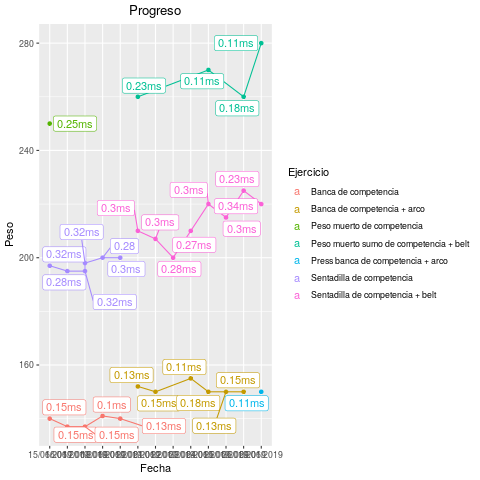
\includegraphics[width=.9\linewidth]{tmp.png}
\end{center}
\end{document}
